\subsection{Forecasts and auxiliary gains on held-out subjects}
\label{app:subject_transfer}

We partitioned the UCI-HAR training subjects by reference and used $3\%$
of each fitting activity's windows as labels. All arms shared an
eight-epoch warm start, Adam state, minibatches and encoder forwards.
During continuation, both arms applied supervised loss to clean and
masked views. Reconstruction trained the same decoder in both arms.
Joint training also passed its gradient to the encoder. Each mask
replaced $25\%$ of the coordinates by their fitting means.

Across eight development splits, none of eight reconstruction,
contrastive or neighborhood-consistency settings reached both the
$0.5$-point activity gain and the $0.98$ auxiliary loss ratio set in advance.
Reconstruction at weight $3$ came closest, with a $0.36$-point gain and a
loss ratio of $0.815$. We used the fixed weight-$0.3$ fallback for the
forecast experiment. Across 16 new references on nine official test
subjects, its reconstruction loss ratio was $0.897$ ($[0.886,0.908]$)
and its activity accuracy changed by $0.06$ points ($95\%$ CI $[-0.17,0.28]$) at the nominal learning rate.

\begin{figure}[t]
\centering
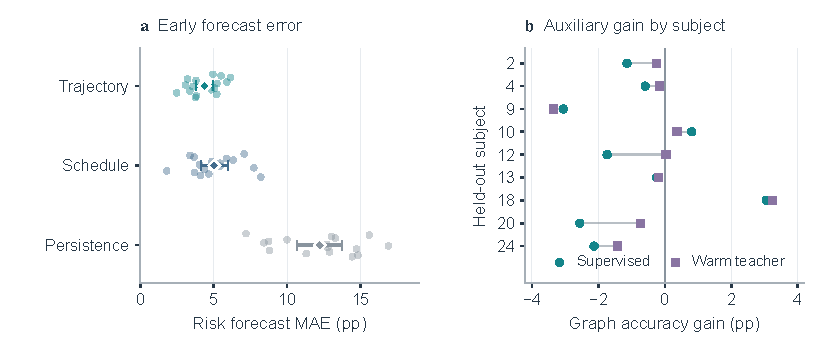
\includegraphics[width=\linewidth]{figures/fig_subject_transfer.pdf}
\caption{Subject-disjoint continuation on UCI-HAR. (a) Error in
forecasting the maximum old-rule disagreement at epoch 24. Each small
point averages eight forecasts from one reference. Diamonds and bars
show means and $95\%$ intervals across references for each estimator.
(b) Accuracy gains from graph-derived targets over the two matched
controls, averaged across references for each of the nine test subjects.}
\label{fig:subject_transfer}
\end{figure}

We fit two frozen readers to the healthy features, for activity and
movement versus rest. For each reader we recorded class decisions and
fixed confidence rules at $80\%$ and $50\%$ healthy coverage. The forecast
uses unlabeled logits at epochs 0, 1 and 3. For each rule it fits terminal
disagreement with a ridge logistic model of the signed preservation
margins, their two changes through epoch 3 and the two observed early
disagreement indicators. For an accepted reference output, the margin
is the smaller of the class margin and the reference class log odds
minus the threshold log odds. For an abstained reference output, the
margin is the threshold log odds minus the current winning class log
odds. The class-only rule uses the class margin.

The schedule estimator knows the objective, learning rate, reader and
rule. It uses the cell's mean terminal disagreement in development.
The trajectory estimator adds the change in mean predicted risk between
that cell and the new monitor. A held-reference calibration selected
the scale of that correction from $\{0,.25,.5,.75,1\}$, choosing $1$.
We refit on all 12 calibration references, then sealed the forecasts
before epoch 4 in each confirmation run. Monitoring and evaluation
subjects were disjoint. The trajectory, schedule and epoch-3 persistence
estimators had mean absolute errors of $4.37$, $5.04$ and $12.23$ points
(Figure~\ref{fig:subject_transfer}a). The paired trajectory improvement
over persistence was $7.85$ points ($[6.10,9.61]$); its improvement over
schedule was $0.67$ ($[-0.38,1.72]$). All $128$ reader--update pairs
exceeded the $5\%$ budget. The trajectory and schedule estimators flagged
all of them, and persistence missed $14$.

For a separate auxiliary, we propagated fitting activity labels over a
30-nearest-neighbor cosine graph~\citep{zhu2003harmonic} and matched its
soft targets on masked unlabeled windows. Controls use supervision alone
or healthy-model soft targets. Graph setup averages $0.51$ CPU seconds.
Weight $0.1$ gains $1.00/2.59$ points over these controls on eight development
splits. On 16 new references across nine official test subjects, it instead
loses $0.82$ points $[-1.52,-0.13]$ versus supervision and $0.22$
$[-0.93,0.49]$ versus the healthy teacher (Figure~\ref{fig:subject_transfer}b).
Intervals vary references on this fixed cohort. Retained healthy forwards
reproduce both old readers' logits bit for bit.

\subsection{Early warning under matched RadioML continuations}
\label{app:rml_trajectory}

We trained an eleven-class modulation reader with $3\%$ of fitting
modulation labels and used signal-to-noise ratio as the auxiliary target.
The detached and joint arms shared their warm model, Adam state and
minibatches at each of three learning rates. We used the same
signed-margin forecast with snapshots at epochs 0, 2 and 6 to predict
epoch-24 risk. Calibration used 12 references. Across 16 new references
and six arms per reference, we sealed forecasts before epoch 7 and
evaluated $4{,}400$ held-out signals per reference.

Trajectory, schedule-only and epoch-6 persistence gave errors of
$2.25$, $2.87$ and $8.27$ points. The paired improvement was $0.62$
points ($95\%$ CI $[0.28,0.96]$) over schedule and $6.02$
($[4.79,7.26]$) over persistence. At a $5\%$ budget, the trajectory
and schedule rules kept the reference for all 96 episodes. Five
would have met the budget with the unchanged reader. Persistence
retained 69 references and violated the budget on 22 episodes.
Keeping the healthy branch exactly reproduced the old logits.

Joint SNR training changed modulation accuracy by $0.05$
($[-0.02,0.11]$), $0.35$ ($[0.20,0.50]$), and $0.13$
($[-0.18,0.43]$) points at rates $10^{-5}$, $10^{-4}$, and $10^{-3}$.
The interval for the middle rate is $[0.16,0.54]$ with a Bonferroni
correction across the three rate-specific contrasts.

\subsection{Choosing a readout repair before continuation ends}
\label{app:rml_early_repair}

In a separate RadioML experiment, we varied three learning rates from
$3\times10^{-6}$ to $10^{-4}$ and added an affine repair. We estimated
the residual between the unchanged reader and the healthy logits on
512 paired unlabeled anchors. Ridge regression predicts that residual
from the current features. The alignment uses a separate anchor set and
adds an affine map to the old output. The current prediction is shared.

For each of 16 new references, we sealed an epoch-six choice for each
of six continuations. The policy takes the first path whose forecast
plus $0.5$ points fits within $5\%$. It tries the unchanged reader,
then alignment, then the exact reference. All policies were evaluated
after epoch 24 on $4{,}400$ held-out signals per reference.

\begin{table}[htbp]
\centering
\caption{Early release decisions on 96 RadioML continuations. Counts
give the number of updates assigned to each path. Violations count
updates exceeding the $5\%$ old-decision budget on held-out signals.
Max is the largest disagreement across updates and rules, in percent.}
\label{tab:rml_early_repair}
\begin{tabular}{lrrrrr}
\toprule
Policy & Direct & Aligned & Reference & Violations & Max \\
\midrule
Schedule, direct only & 0 & 0 & 96 & 0 & 0.00 \\
Trajectory, direct only & 6 & 0 & 90 & 0 & 3.84 \\
Persistence with alignment & 59 & 16 & 21 & 39 & 9.77 \\
Schedule with alignment & 0 & 64 & 32 & 3 & 7.57 \\
Trajectory with alignment & 6 & 57 & 33 & 2 & 6.70 \\
\bottomrule
\end{tabular}
\end{table}
Alignment reduced trajectory-based reference retention from $90$ to $33$ of 96 updates, with $2$ budget violations. The schedule policy with alignment retained $32$ references and had $3$ violations. At rate $10^{-4}$, the joint SNR arm changed modulation accuracy by $0.24$ points ($[0.05,0.42]$).
Both violations were class changes. Without alignment, early monitoring
released six updates with no violations, while schedule retained all 96.
At the middle rate, all 32 continuations retained the reference under
the three-path trajectory policy, including the joint runs with a
confirmed accuracy gain.
